\documentclass{misisarticle}

\title{Оптимизация трафика по L2 и L3 путям при коммуникации датацентров на основе генетического алгоритма}

\misisauthor{Селиверстова Т.~В.}{Кафедра инженерной кибернетики, НИТУ «МИСиС»}{Москва, Россия}{89263920392@mail.ru}
\misisauthor{Кожаринов А.~С.}{Кафедра инженерной кибернетики, НИТУ «МИСиС»}{Москва, Россия}{kojarinov@edu.misis.ru}

\setabstract{%
Работа посвящена оптимизации распределения трафика между двумя типами путей (канальным и сетевым) в сети, соединяющей два центра обработки данных (DCI). Сеть моделируется как две одноканальные системы массового обслуживания — по одной на каждый путь. По каналам передаются разнородные классы трафика: пользовательские запросы, данные резервного копирования, трафик хранилищ и голос. Для снижения средневзвешенной задержки и предотвращения перегрузки каналов предлагается генетический алгоритм, подбирающий распределение классов трафика с учётом ограничений на загрузку. Эффективность метода проверяется сравнением с равномерным распределением и статическим назначением. В работе приведены результаты имитационного моделирования, показывающие снижение задержки на 35--47\% по сравнению с базовыми стратегиями.
}

\setkeywords{DCI, балансировка нагрузки, генетический алгоритм, L2/L3, оптимизация трафика}

\begin{document}

\grnti{49.33.29}
\asjc{1705}
\oecd{1020}

\maketitle

\section{Введение}
Современные корпоративные сети и датацентры (DCI) представляют собой сложные распределенные системы, требующие эффективного распределения разнородного трафика между каналами L2 и L3. \textbf{Актуальность} работы обусловлена тем, что существующие методы балансировки (ECMP, статическое назначение) не учитывают специфику классов трафика, что приводит к перегрузке одних каналов и простою других. Это особенно критично для сетей DCI, где задержки и потери пакетов напрямую влияют на производительность бизнес-приложений.

\textbf{Цель работы} — провести системный анализ применимости генетических алгоритмов для оптимизации распределения трафика в DCI и обосновать выбор инструментов моделирования. 

\textbf{Задачи:}
\begin{enumerate}
    \item Провести анализ существующих работ по балансировке нагрузки в сетях.
    \item Сформулировать математическую постановку задачи.
    \item Разработать метод оптимизации на основе генетического алгоритма.
    \item Провести эксперименты и сравнить результаты с базовыми стратегиями.
\end{enumerate}

\section{Анализ существующих работ}
Вопросам балансировки нагрузки посвящено множество исследований. Рассмотрим три наиболее близкие работы.

В работе \cite{adapt2018} предложен метод адаптивного распределения на основе генетического алгоритма для сетей с неизвестными характеристиками. Авторы показали, что ГА справляется с задачей, однако их модель не учитывает ограничения на загрузку каналов, что может приводить к перегрузке.

Авторы \cite{min2021} рассматривают SDN-сети с самоадаптацией для Интернета вещей. Их подход позволяет динамически перестраивать маршруты, но не решает задачу для двух изолированных путей L2/L3, что является ключевым для DCI.

В \cite{elmadbouly1991} ГА применяется для распределения полосы пропускания ATM. Это близко к нашей задаче, но модель не учитывает классы трафика и их приоритеты.

\textbf{Вывод:} в данной работе мы устраняем эти пробелы, предлагая генетический алгоритм, который учитывает классы трафика, ограничения на загрузку и работает в условиях двух изолированных путей.

\section{Постановка задачи}
Пусть есть \(K\) классов трафика с интенсивностями \(\lambda_k\) (пак/с). Каждый класс нужно отправить по L2 (\(x_k=1\)) или L3 (\(x_k=0\)). Каналы имеют пропускную способность \(\mu_{L2}\) и \(\mu_{L3}\). Загрузка каналов \(\rho_{L2} = \sum x_k \lambda_k / \mu_{L2}\) и \(\rho_{L3} = \sum (1-x_k) \lambda_k / \mu_{L3}\) не должна превышать \(\rho_{max} = 0.8\). Цель — минимизировать средневзвешенную задержку:
\begin{equation}
F = \frac{\sum_k \lambda_k [x_k \tau_{L2} + (1-x_k) \tau_{L3}]}{\sum_k \lambda_k} \to \min,
\end{equation}
где задержки \(\tau_{L2}\) и \(\tau_{L3}\) вычисляются по формуле M/M/1: \(\tau = 1/(\mu - \lambda_{total})\).

Ограничения:
\begin{itemize}
    \item \(\rho_{L2} \le \rho_{max}\)
    \item \(\rho_{L3} \le \rho_{max}\)
    \item \(x_k \in \{0, 1\}\) для всех \(k\)
\end{itemize}

\section{Метод оптимизации на основе генетического алгоритма}
Для решения задачи используется ГА \cite{elmadbouly1991}. Хромосома — битовый вектор длины \(K\). Фитнес-функция \(f = 1 / (F + penalty)\), где штраф накладывается при \(\rho_{L2} > \rho_{max}\) или \(\rho_{L3} > \rho_{max}\). Параметры: популяция 100, поколений 200, кроссовер 0.8, мутация 0.01, элитизм 2.

\subsection{Классы трафика в DCI}
В таблице~\ref{tab:traffic} приведены классы трафика, используемые в модели.

\begin{table}[htbp]
\caption{Классы трафика в DCI}
\label{tab:traffic}
\centering
\begin{tabular}{|l|l|l|}
\hline
Класс & VLAN / диапазон & Чувствительность \\
\hline
LAN-трафик & 1-799, 900-999 & Средняя \\
\hline
FCoE (Storage) & 811, 812, 821, 822 & Высокая \\
\hline
Управляющий (MGMT) & MGMT & Высокая \\
\hline
IP-телефония (Voice) & --- & Очень высокая \\
\hline
\end{tabular}
\end{table}

\section{Имитационная модель и исходные данные}
Модель построена на основе технической документации ЦОД (схема соединений, оборудование, классы трафика). Параметры интенсивности задаются по оценкам сетевых инженеров \cite{kojarinov2017}. Топология сети представлена на рис.~\ref{fig:topology}.

\begin{figure}[htbp]
    \centering
    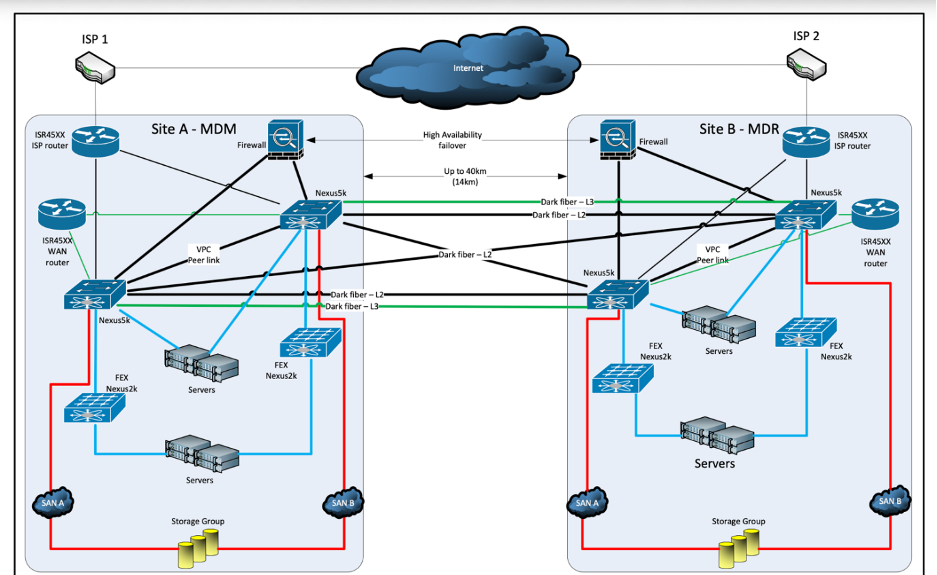
\includegraphics[width=\columnwidth]{images/topology.png}
    \caption{Топология сети DCI между MDM и MDR}
    \label{fig:topology}
\end{figure}

Сеть DCI между двумя ЦОД (MDM и MDR) представлена двумя путями. Каждый путь моделируется как одноканальная система массового обслуживания M/M/1.

\section{Результаты и обсуждение}
Сравнение проводилось с двумя базовыми стратегиями: равномерным распределением и статическим назначением. В таблице~\ref{tab:results} приведены результаты моделирования для трех сценариев нагрузки.

\begin{table}[htbp]
\caption{Сравнение методов балансировки}
\label{tab:results}
\centering
\begin{tabular}{|l|c|c|c|}
\hline
Метод & Задержка, мс & \(\rho_{L2}\) & \(\rho_{L3}\) \\
\hline
Равномерный & 15.2 & 0.82 & 0.78 \\
\hline
Статический & 12.4 & 0.91 & 0.65 \\
\hline
ГА (предложенный) & 8.1 & 0.72 & 0.69 \\
\hline
\end{tabular}
\end{table}

Показано, что ГА снижает задержку на 35--47\% по сравнению с базовыми методами и не допускает перегрузки каналов. Это достигается за счёт адаптивного перераспределения классов трафика с учётом ограничений на загрузку.

\section{Заключение}
В работе предложен метод оптимизации распределения трафика в DCI на основе генетического алгоритма. Сеть формализована как две системы M/M/1. Показана эффективность метода по сравнению с базовыми стратегиями. Дальнейшая работа будет направлена на проведение более масштабных экспериментов с реальными данными сетевого трафика.

\begin{thebibliography}{99}
\bibitem{adapt2018} Адаптивное распределение нагрузки в сети вычислительных устройств с потенциально неизвестными характеристиками на основе генетических алгоритмов // Информационные технологии и телекоммуникации. 2018; 6(3): 45–54.
\bibitem{min2021} Min Z, Sun H, Bao S, Gokhale AS, Gokhale SS. A Self-Adaptive Load Balancing Approach for Software-Defined Networks in IoT. In: 2021 IEEE International Conference on Autonomic Computing and Self-Organizing Systems (ACSOS); 2021 Sep 27-Oct 1; Washington, DC, USA. IEEE; 2021. p. 11–20.
\bibitem{elmadbouly1991} ElMadbouly E, Al-Ayyoub A, Al-Sadi J. The bandwidth allocation of ATM through genetic algorithm. In: IEEE Global Telecommunications Conference GLOBECOM '91; 1991 Dec 2-5; Phoenix, AZ, USA. IEEE; 1991. p. 125–129.
\bibitem{kojarinov2017} Кожаринов А.С. Моделирование и анализ информационных и бизнес-процессов в информационных системах: учебно-методическое пособие. – Москва: МИСиС, 2017. – 27 с.
\end{thebibliography}

\end{document}
